% Companion note for the GFOR (grid-forming VSC) injector model in RAMSES.
% Based on the model notes by T. Van Cutsem (July 2026) and the CODEGEN
% description file inj_GFOR.txt in the RAMSES repository.
% Compile with:  pdflatex inj_gfor.tex  (twice)
\documentclass[11pt,a4paper]{article}
\usepackage[margin=25mm]{geometry}
\usepackage{amsmath,bm}
\usepackage{graphicx}
\usepackage[T1]{fontenc}
\renewcommand{\familydefault}{\sfdefault}
\setlength{\parindent}{0pt}
\setlength{\parskip}{2ex}
\pagestyle{empty}

\begin{document}

\begin{center}
{\large\bf GFOR: Grid-forming VSC modelling in RAMSES}\\[1ex]
{\small based on the model by T.\ Van Cutsem (July 2026)}
\end{center}

{\bf Overview.} An MMC-type converter connected to the grid through its
transformer (resistance $R$, inductance $L$, ideal ratio $r$; no LC filter).
The DC side of the VSC is not modelled ($v_{dc}$ is assumed constant); the
focus is on the AC grid dynamics. Per-unit values refer to the nominal
apparent power $S_{nom}$ of the converter; the conversion factor of currents
is $k = r\,S_{base}/S_{nom}$.

{\bf Reference frame.} The $d$ axis is attached to the internal phase angle
$\delta_m$ of the modulated voltage:
\begin{align*}
v_d &= v_x\cos\delta_m + v_y\sin\delta_m, & v_q &= -v_x\sin\delta_m + v_y\cos\delta_m
\end{align*}
and similarly for the converter-side currents $i_{xt}=k\,i_x$, $i_{yt}=k\,i_y$.
The voltage-current relationship in the transformer, in the $d$-$q$ frame, is:
\begin{align*}
v_{md} &= \frac{v_d}{r} + R\, i_d - \omega_m L\, i_q, &
v_{mq} &= \frac{v_q}{r} + R\, i_q + \omega_m L\, i_d
\end{align*}

{\bf Active power and phase angle control.} ``Virtual synchronous machine''
with inertia emulation ($H$) and oscillation damping ($D$):
\[
2H\frac{d\omega_m}{dt} = P^\ast - P_{virt} - D\,(\omega_m - \tilde\omega_g)
 + \frac{1-\omega_m}{R_{droop}},
\qquad
\frac{d\delta_m}{dt} = \omega_N(\omega_m - \omega_{ref})
\]
\begin{center}
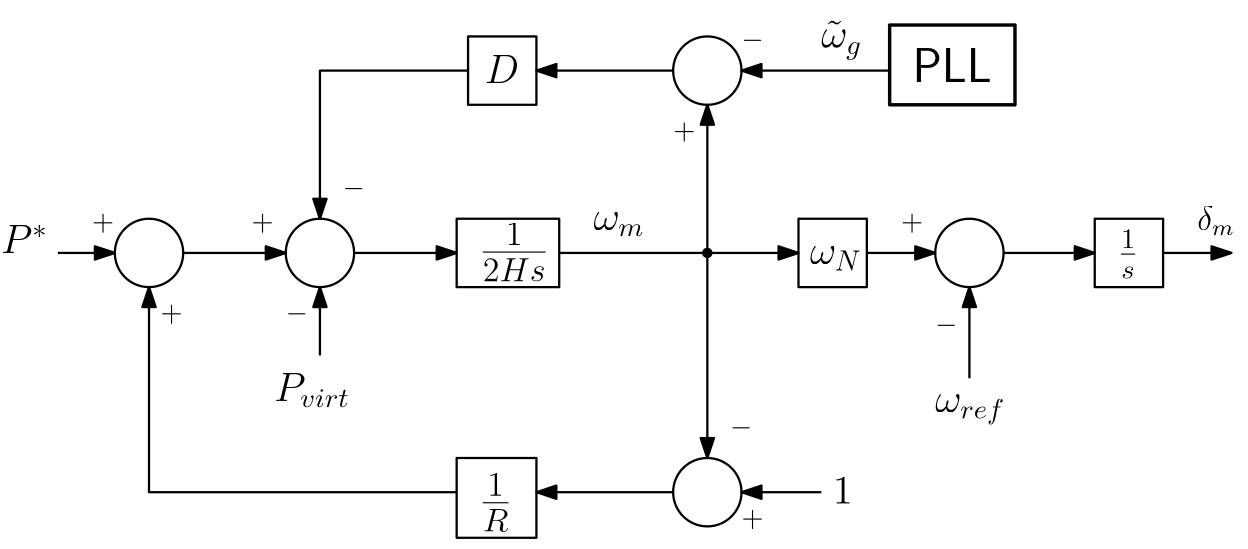
\includegraphics[width=0.75\textwidth]{inj_gfor_vsm.png}
\end{center}
$P_{virt} = (v_d/r)\, i_d^{*} + (v_q/r)\, i_q^{*}$ is the ``virtual power''
computed from the unsaturated currents. It amounts to the active power $P$
when the current is not limited, and yields improved large-disturbance
stability under limitation of the current. Participation in primary frequency
control is optional, with droop $R_{droop}$ (a very large value disables it).

{\bf PLL.} The purpose of the PLL is only to estimate the grid angular
frequency $\tilde\omega_g$ for the damping term. Same model as in the
grid-following converter (see the GFOL note), with gains
$K_{p\omega}=10/(\omega_N T_{pll})$ and $K_{i\omega}=25/(\omega_N T_{pll}^2)$,
$\omega_N = 2\pi f_N$. The PLL is frozen when the PCC voltage falls below
0.4~pu and reactivated above 0.5~pu (fixed thresholds, with hysteresis).

{\bf Current limitation.} The currents $(i_d^{*}, i_q^{*})$ that would result
from normal voltage control ($v_{md}=V_m^0$, $v_{mq}=0$) are determined from:
\[
V_m^0 = \frac{v_d}{r} + R\, i_d^{*} - \omega_m L\, i_q^{*},
\qquad
0 = \frac{v_q}{r} + R\, i_q^{*} + \omega_m L\, i_d^{*}
\]
The overload ratio $\rho = \sqrt{(i_d^{*})^2+(i_q^{*})^2}\,/\,I_{max}$ is
passed through a first-order lag of time constant $T_e$ (typically 1~ms) with
a non-windup lower limit of 1, giving $\rho_s$. Both components are decreased
in the same proportion, and the modulated voltage is set to the value that
yields the saturated currents:
\[
i_{ds}^{*} = i_d^{*}/\rho_s, \quad i_{qs}^{*} = i_q^{*}/\rho_s,
\qquad
v_{md} = \frac{v_d}{r} + R\, i_{ds}^{*} - \omega_m L\, i_{qs}^{*},
\quad
v_{mq} = \frac{v_q}{r} + R\, i_{qs}^{*} + \omega_m L\, i_{ds}^{*}
\]
\begin{center}
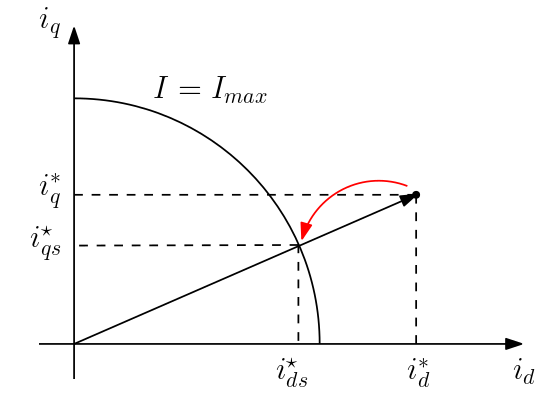
\includegraphics[width=0.42\textwidth]{inj_gfor_currentlim.png}
\end{center}
If $I < I_{max}$: $\rho_s = 1$, $i_d^{*}=i_{ds}^{*}=i_d$,
$i_q^{*}=i_{qs}^{*}=i_q$, $v_{md}=V_m^0$ and $v_{mq}=0$.

\newpage

{\bf Data.} The record has the following structure (defaults from the
{\tt Benchmark\_1\_VSC} test case distributed with RAMSES):

{\tt INJEC GFOR NAME BUS FP FQ P Q\ \ R L r Snom H D Tpll Rdroop Imax Te ;}

\begin{center}
\begin{tabular}{llll}
\hline
Parameter & Description & Unit & Default \\
\hline
{\tt R}      & resistance of connection transformer            & pu  & 0.005 \\
{\tt L}      & inductance of connection transformer            & pu  & 0.15  \\
{\tt r}      & ratio of ideal transformer                      &     & 1.02  \\
{\tt Snom}   & nominal apparent power                          & MVA & 1100  \\
{\tt H}      & inertia constant                                & s   & 5.0   \\
{\tt D}      & damping constant of virtual synchronous machine &     & 300   \\
{\tt Tpll}   & time constant of PLL                            & s   & 0.1   \\
{\tt Rdroop} & droop of primary frequency control              & pu  & 999   \\
{\tt Imax}   & maximum current (typically 1--1.2)              & pu  & 1.0   \\
{\tt Te}     & time constant of current saturation             & s   & 0.001 \\
\hline
\end{tabular}
\end{center}

The setpoints $V_m^0$ ({\tt Vmo}) and $P^\ast$ ({\tt Po}) are computed at
initialization from the power-flow solution and can be modified during the
simulation with {\tt CHGPRM} disturbances.

Example (from {\tt Benchmark\_1\_VSC}):

{\tt INJEC GFOR HVDC A 1. 1. 0. 0. 0.005 0.15 1.02 1100. 5.0 300. 0.100 999. 1.0 0.001 ;}

{\bf Observables:} {\tt P}, {\tt Pvirt}, {\tt Q}, {\tt Vm}, {\tt vmd},
{\tt vmq}, {\tt deltam}, {\tt omegam}, {\tt w\_pll}, {\tt I}, {\tt id},
{\tt id*}, {\tt id*s}, {\tt iq}, {\tt iq*}, {\tt iq*s}, {\tt rho}, {\tt rhos}.

\end{document}
